\chapter{Applicazione Mobile}\label{chap:mobile-app}

In questo capitolo verrà presentato un esempio di applicazione mobile in grado di connettersi al \emph{City Service} e di eseguire le operazione di prenotazione e ritiro delle ricariche. Il suo scopo è permettere all'utente di interagire con la smart-city al fine di ridurre le problematiche derivanti dall'utilizzo di veicoli elettrici. La comunicazione avviene mediante i protocolli visti nella Sez. ~\ref{sec:protocol}.

Inizialmente era possibile eseguire solo operazioni di prenotazione e cancellazione di ricariche e funzionava unicamente in presenza del simulatore in quanto si prendeva il possesso di un veicolo simulato. Il funzionamento è stato poi ampliato con la possibilità di connettersi tramite Bluetooth a un veicolo reale, opportunità concessa dal \emph{Centro Ricerche Fiat} (\emph{CRF}), oppure di connettersi in assenza di veicoli per permettere all'utente di effettuare una ricarica comodamente seduto a casa.

A questo si è aggiunta la possibilità di analizzare il profilo altimetrico che separa il dispositivo mobile da un determinato EVSE con lo scopo di fare previsioni più accurate sui consumi necessari a raggiungerlo.

La piattaforma di sviluppo scelta è \emph{Android} vista la sua grandissima diffusione e versatilità.

\section{Funzionalità}



\section{Architettura}

La piattaforma scelta per lo sviluppo è Android dalla versione \emph{4.0.3} in su. Questo perché vanta maggiori performance e un interfaccia utente più gradevole è facile da programmare. La libreria di base per interfacciarsi con il SIB è quella esposta nella sezione ~\ref{subsec:ioe-lib}.

La comunicazione con il servizio cittadino avviene tramite scambio di messaggi con il \emph{City SIB}, mentre le informazioni relative al veicolo, in particolar modo se quest'ultimo è simulato, arrivano dal \emph{Dash SIB}. È possibile collegare l'applicazione ad un veicolo reale che sia provvisto della tecnologia Blue\&{}Me di Fiat. I dati del profilo altimetrico sono ottenuti tramite una libreria, chiamata \emph{UniboGeoTools}, che ho sviluppato appositamente per l'occasione.

\subsection{Android}

Malgrado Android sia ampiamente conosciuto penso sia necessario spendere qualche parola al fine di introdurre i concetti che stanno alla base della programmazione di applicazioni su questo sistema operativo per poter capire approfonditamente il resto della trattazione.

Android è un sistema operativo basato Linux-based, Open Source, orientato all'utilizzo su dispositivi mobili anche se negli ultimi anni sta prendendo sempre più piede all'interno di smart-tv, dispositivi embedded, mini computer ecc..

La programmazione di applicazioni avviene attraverso una versione ad-hoc del linguaggio Java che, seppur venga eseguita su una virtual machine diversa dalla JVM (Dalvik), ne mantiene quasi tutte le caratteristiche e la libreria di base. Naturalmente oltre alla libreria standard vengono fornite le API che permettono l'interfacciamento con le funzionalità di Android.

\subsubsection{Activity}

Le Activity sono uno degli elementi centrali della programmazione di applicazioni Android (\cite{html:android}). In genere un Activity rappresenta una singola schermata della nostra applicazione. Le applicazioni possono definire una o più Activity per trattare diverse fasi del software, e generalmente ognuna di esse corrisponde ad un azione specifica che può essere eseguita dall'utente. 

Ci può essere una sola Activity attiva in un determinato istante, quelle che invece non sono attive possono essere terminate in qualunque momento dal sistema operativo al fine di recuperare memoria, questo comporta che il programmatore debba prevedere per ogni Activity il codice necessario a salvarne lo stato per permetterne il ripristino nel caso sia necessario. Questo comporta, come si può vedere in figura ~\ref{fig:android-activity}, che le Activity di Android abbiano un ciclo di vita abbastanza complesso. 

\subsubsection{Service}

Un Service è un processo che gira in background (un concetto molto simile al deamon in ambiente Unix) e può essere vviato e comandato da Activity o altri Service. La classe Service viene utilizzata per creare componenti software che possono svolgere attività in modo ``invisibile'', senza interfaccia utente.

Un Service può trovarsi in due stati(\cite{emanuele:android}):

\begin{itemize}
	\item \textbf{Started}: Un servizio si trova in questo stato quando viene invocato il metodo startService(), il servizio gira in background per un tempo indefinito o finché il componente che lo ha invocato non viene distrutto (Fig. ~\ref{fig:android-service} sinistra).
	\item \textbf{Bounded}: Un servizio si trova in questo stato quando si invoca il metodo bindService(). I servizi di questo tipo offrono un'interfaccia per la comunicazione client-server, in questo modo le componenti che invocano il servizio possono interagire con esso. In questo caso il servizio è attivo solo finché le componenti sono associate con esso (Fig. ~\ref{fig:android-service} destra).
\end{itemize}

\noindent
Un Servizio avviato ha una priorità più alta rispetto ad Activity in stato di inattività, in questo modo vi è minore probabilità per un Service di essere terminato dal gestore delle risorse di runtime. L’unica ragione per cui Android potrebbe fermare un Service prematuramente è per fornire risorse addizionali al componente software in primo piano (normalmente una Activity).

I servizi vengono avviati nel thread principale del processo, ciò significa che se eseguissero operazioni bloccanti o ad alto consumo di risorse potrebbero portare al blocco dell'intero processo e far generare ad Android un errore del tipo: ``Application Not Responding'', per evitare questo è bene far gestire il servizio in un thread separato.

\begin{figure}[H]
        \centering
        \begin{subfigure}[b]{0.49\textwidth}
			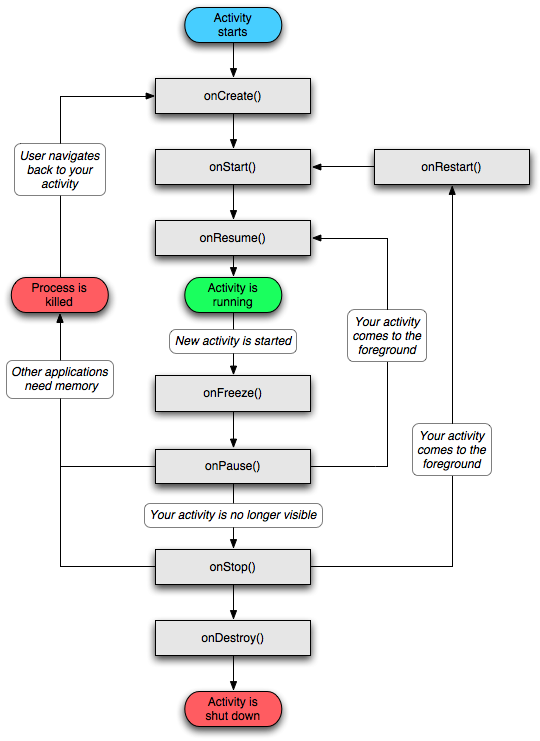
\includegraphics[width=\textwidth]{assets/android-activity.png}
			\caption{Ciclo di vita di un Activity Android}
			\label{fig:android-activity}
		\end{subfigure}
        \begin{subfigure}[b]{0.49\textwidth}
			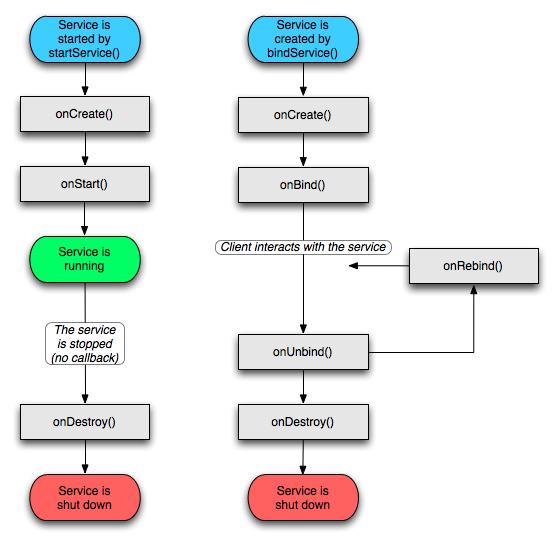
\includegraphics[width=\textwidth]{assets/android-service.png}
			\caption{Ciclo di vita di un Service Android}
			\label{fig:android-service}
		\end{subfigure}
        \caption{Ciclo di vita Activity e Service Android}
\end{figure}

\subsection{Blue\&{}Me}

Il Blue\&{}Me è il risultato di un accordo tra Fiat Auto e Microsoft con l'obiettivo di progettare sistemi telematici innovativi per l'automotive, il sistema è stato presentato nel 2006 (\cite{al2012android}). Basato sulla piattaforma Windows Embedded Automotive (unione del sistema operativo Windows CE con il middleware Microsoft Auto) è sviluppato da Magneti Marelli (azienda del gruppo FIAT) in collaborazione con Microsoft (\cite{wiki:blue-me}).

Blue\&{}Me è un sistema viva voce con tecnologia Bluetooth, riconoscimento vocale, lettore multimediale con presa USB e comandi al volante. Fiat Auto e Microsoft, con il supporto di Magneti Marelli, offrono una piattaforma adattabile alla maggior parte dei telefoni cellulari e lettori musicali. Il sistema si interfaccia al cellulare mediante la tecnologia Bluetooth e permette al guidatore di rispondere al telefono lasciando il telefono in tasca. 

La funzionalità del Blue\&{}Me più importante ai nostri scopi è la possibilità di monitorare i parametri del veicolo. Nel nostro caso abbiamo lavorato con un prototipo di Fiat Daily elettrico opportunamente modificato per trasmettere i dati della batteria tramite tecnologia Bluetooth. La connessione è stata possibile grazie a delle librerie fornite dal CRF con tanto di applicazione di esempio.

L'interazione con il Blue\&{}Me è di tipo push ovvero ogniqualvolta che la centralina della macchina si accorge che un dato è variato (secondo una determinata soglia) allora lo ``scrive'' sull'interfaccia Bluetooth. Il che implica che se dall'altra parte ci deve essere un applicazione che dedica un processo alla sola lettura delle informazioni che arrivano dal Blue\&{}Me. Fiat, nella libreria fornita, mette a disposizione un Service Andorid adatto allo scopo.

\subsection{Operazioni Asincrone}

Tutte le operazioni che prevedono l'utilizzo della rete, quindi potenzialmente lunghe, sono eseguite all'interno di un \code{AsyncTask} ovvero una classe messa a disposizione dalla libreria di base di Android che permette di eseguire operazioni asincrone e contemporaneamente aggiornare l'interfaccia grafica. Questo da un lato permette di avere un applicazione fluida in quanto l'interfaccia non rimane bloccata in attesa dei risultati e dall'altro evita il verificarsi di errori dovuti al fatto che Android non permette di modificare l'interfaccia da un thread diverso da quello destinato al disegno di quest'ultima.

La maggior parte delle operazioni effettuate tramite rete, quindi nel nostro caso scambio di dati con i SIB, reperisce liste di elementi (veicoli, utenti, prenotazioni ecc..) che vengono mostrate all'interno di un apposita tipologia di Activity di Android le \code{ListActivity}.

Al fine di semplificare la programmazione delle Activity che contengono liste i quali elementi sono reperiti tramite la rete, ho creato la classe \code{ListLoaderTask<T>} che ne facilita il caricamento asincrono.

\subsection{Profilo Altimetrico e Contributo Energetico}

Grazie allo sviluppo di un apposita libreria, UniboGeoTools (App. ~\ref{app:unibo-geo-tools}) l'applicazione è in grado di prelevare i dati relativi al profilo altimetrico che separa l'utente da una determinata destinazione e quindi fare uno studio sul contributo energetico necessario a vincere il dislivello. Le informazioni riguardo al consumo energetico sono approssimative ma danno comunque un indicazione valida all'utente il quale se vede che l'energia necessaria a vincere il dislivello è maggiore di quella contenuta nella batteria allora saprà per certo che in quel determinato punto non ci potrà arrivare.

La libreria UniboGeoTools possiede anche funzioni utili a trovare il percorso, in strada, tra due punti. Queste si sono rivelate particolarmente utili al fine di mostrare i percorsi sulla mappa e la distanza precisa che separa l'utente, ad esempio, da una colonnina di ricarica.


\section{Modalità di esecuzione}

L'applicazione al fine di adattarsi ai diversi scenari possibili offre molteplici modalità di esecuzione, questo per adattarsi a tutti gli scenari possibili. La scelta della modalità di esecuzione avviene nella schermata iniziale come si può vedere in figura ~\ref{fig:main-activity}


\begin{figure}
	\centering
	\begin{subfigure}{0.45\textwidth}
		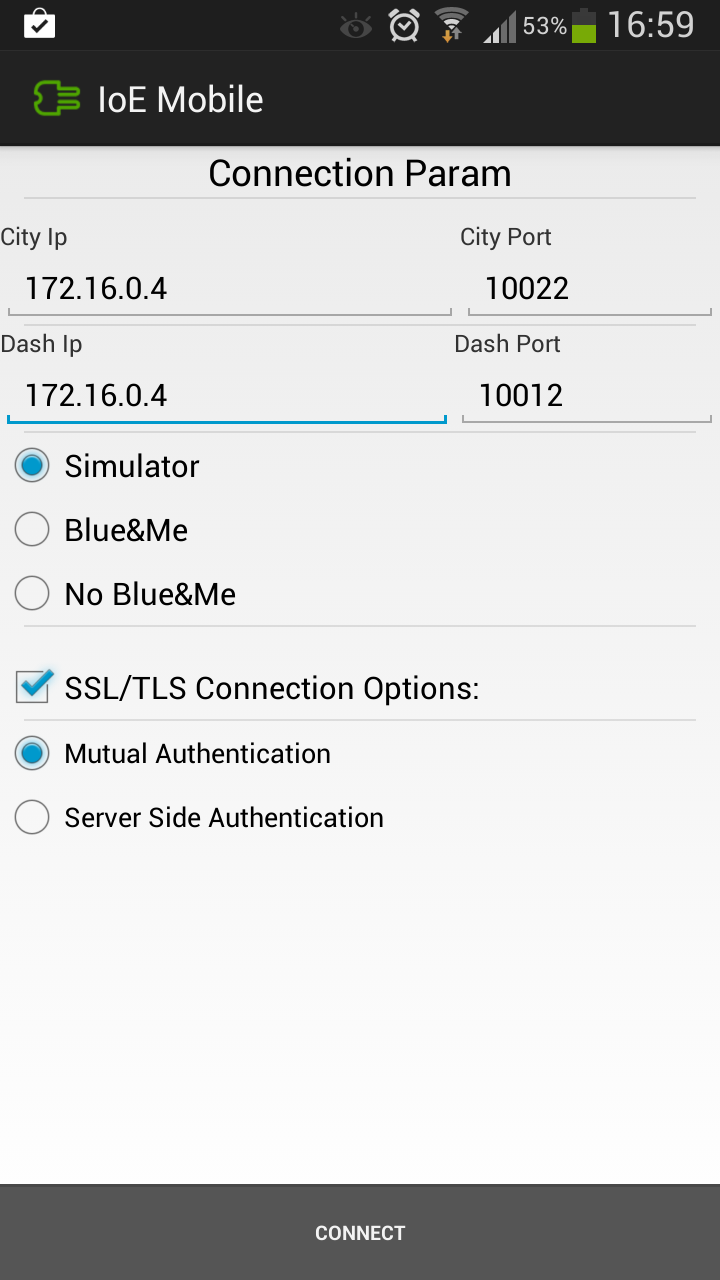
\includegraphics[width=\textwidth]{assets/mobile-app-main.png}
		\caption{Schermata Principale}
		\label{fig:main-activity}
	\end{subfigure}
	\begin{subfigure}{0.45\textwidth}
		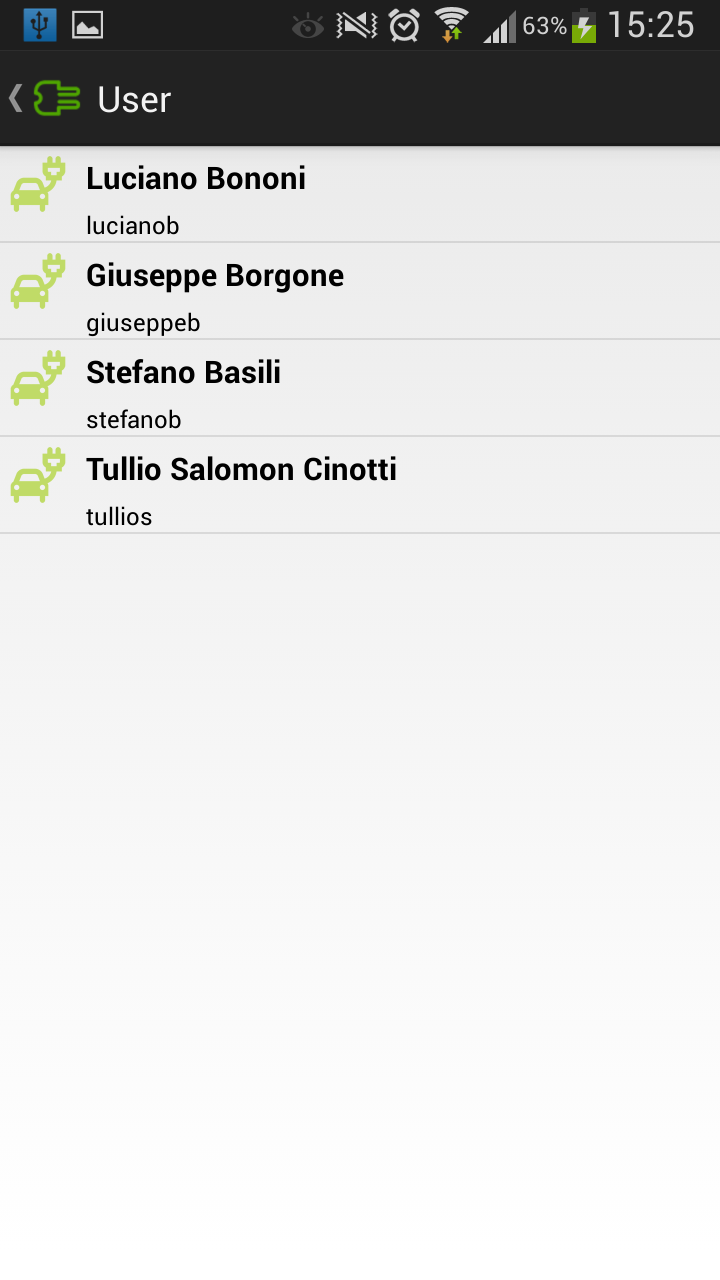
\includegraphics[width=\textwidth]{assets/mobile-app-select-user.png}
		\caption{Selezione Utente}
		\label{fig:select-user}
    \end{subfigure}
    	\begin{subfigure}{0.45\textwidth}
		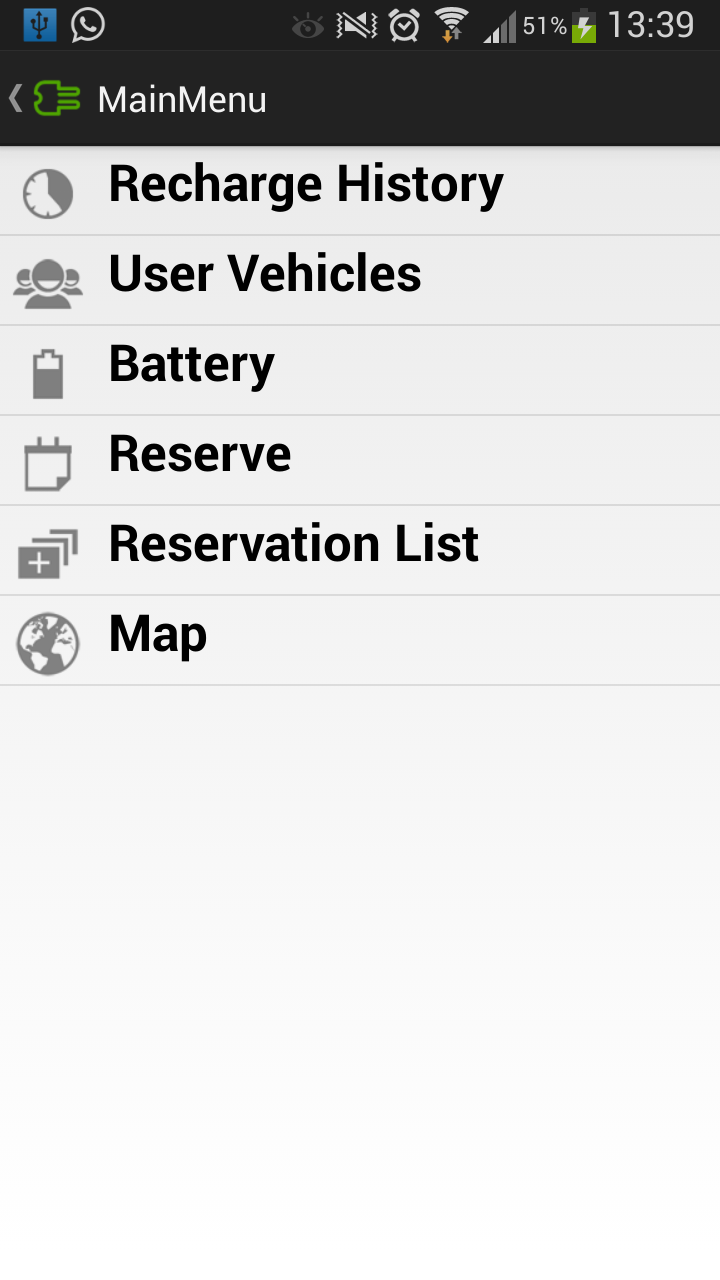
\includegraphics[width=\textwidth]{assets/mobile-app-main-menu.png}
		\caption{Menu Principale}
		\label{fig:main-menu}
	\end{subfigure}
	\begin{subfigure}{0.45\textwidth}
		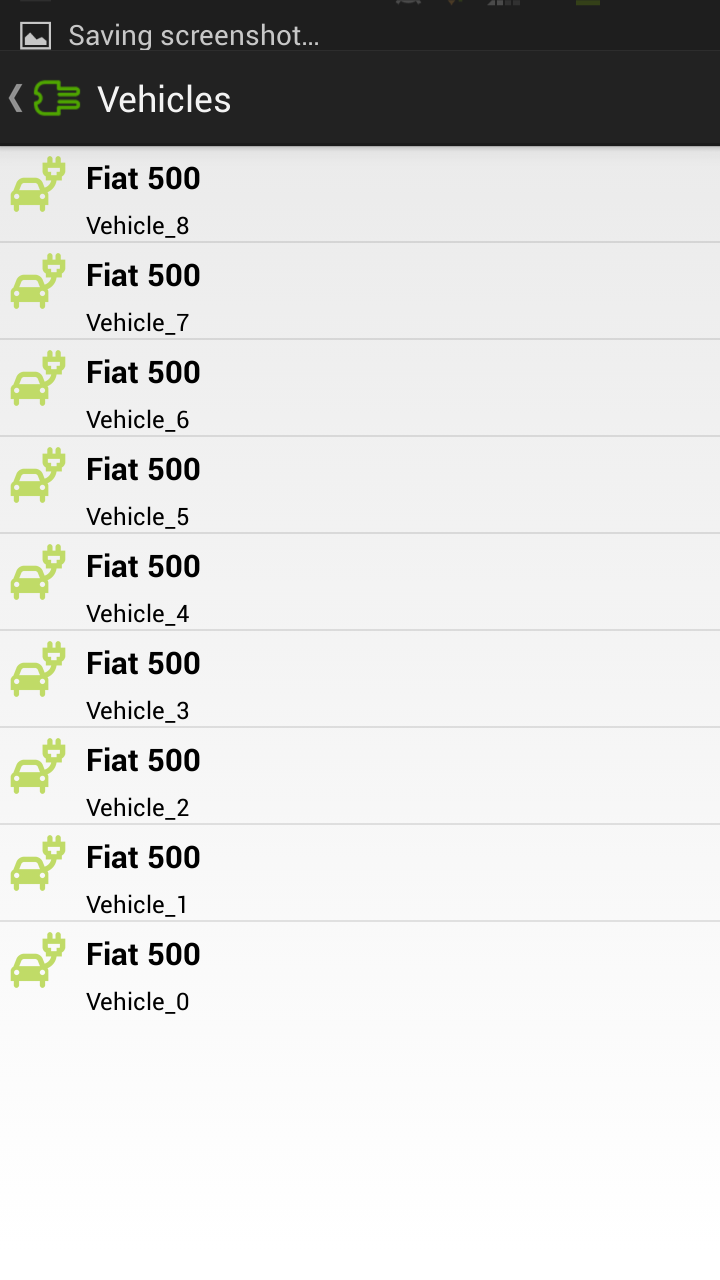
\includegraphics[width=\textwidth]{assets/mobile-app-select-veh.png}
		\caption{Selezione Veicolo}
		\label{fig:select-veh}
    \end{subfigure}
\end{figure}

\subsection{Simulazione}

Questa modalità permette di prendere il controllo di un veicolo contenuto nel simulatore, il quale deve essere avviato con un apposito parametro che causa la scrittura dei dati relativi ai veicoli sul \emph{Dash SIB}. Questo implica che una volta premuto sul pulsante \emph{Connect} (Fig. ~\ref{fig:main-activity}), bisogna scegliere "Luciano Bononi" in quanto è l'utente di default usato dalle macchine del simulatore (Fig. ~\ref{fig:select-user}). Da qui in poi l'applicazione non ha molte differenze rispetto alla modalità di esecuzione con Blue\&{}Me se non che le azioni intraprese avranno ripercussioni sul simulatore e non sul mondo reale.

%\begin{figure}[H]
%        \centering
%        \begin{subfigure}[H]{0.3\textwidth}
%                \adjincludegraphics[width=\textwidth,trim={0 {0.5\height} 0 0},clip]{assets/mobile-app-select-user.png}
%                \caption{Selezione Utente.}
%                \label{fig:select-user}
%        \end{subfigure}%
%        ~ %add desired spacing between images, e. g. ~, \quad, \qquad etc.
%          %(or a blank line to force the subfigure onto a new line)
%        \begin{subfigure}[H]{0.3\textwidth}
%                \adjincludegraphics[width=\textwidth,trim={0 {0.5\height} 0 0},clip]{assets/mobile-app-main-menu.png}
%                \caption{Menu principale senza nessun veicolo selezionato}
%                \label{fig:main-menu}
%        \end{subfigure}
%        \begin{subfigure}[H]{0.3\textwidth}
%                \adjincludegraphics[width=\textwidth,trim={0 {0.5\height} 0 0},clip]{assets/mobile-app-select-veh.png}
%                \caption{Selezione veicolo}
%                \label{fig:select-veh}
%        \end{subfigure}
%        \caption{Schermate Applicazione Mobile}
%\end{figure}

\subsection{Con Blue\&{}Me}

Questa modalità viene usata in un contesto reale e necessita la presenza di un veicolo che possegga la tecnologia Blue\&{}Me di Fiat. Le informazioni relative alla batteria vengono prelevate tramite Bluetooth scritte nel \emph{Dash SIB} per i motivi di interoperabilità spiegati nella Sez. ~\ref{subsec:dash-sib} ovvero dare la possibilità a chiunque di interfacciarsi con l'applicazione mobile a patto di scrivere un adattatore che scriva i dati sulla \emph{Dash SIB}. Le informazioni relative al GPS, siccome non fornite dal veicolo, vengono prelevati dal GPS (o altre fonti) fornito dallo smartphone.

\subsection{Senza Blue\&{}Me}\label{subsec:noblueme}

Questa modalità d'uso è rivolta principalmente a chi vuole svolgere le attività di interazione con il \emph{City Service} senza essere a bordo del proprio veicolo. Questo comporta l'assenza della \textsc{Dash SIB}, infatti quando viene scelta viene disabilitato l'inserimento dei parametri di quest'ultima. Diviene quindi impossibile monitorare i parametri del veicolo e di conseguenza parte del menu principale viene disabilitata. Anche se la \emph{Dash SIB} fosse situata sul cellulare anziché sul veicolo a poco servirebbe in quanto il veicolo sarebbe comunque fuori portata o comunque spento. Si possono comunque svolgere le operazioni di prenotazione e ritiro delle ricariche e tenere monitorato lo stato di quelle già effettuate nonché guardare la mappa con le colonnine.


\section{Funzionalità}

In questa sezione eseguirò un analisi dettagliata delle funzionalità dell'applicazione. La descrizione cercherà di essere il più possibile funzionalità-centrica e non activity-centrica anche se spesso le due cose coincidono. Questo significa che a partire dalle funzionalità cercherò di introdurre le Activity coinvolte nello svolgimento.
Le Activity si trovano nel package \code{it.unibo.ioe.activities}, nel package \code{it.unibo.ioe.activities.maps} invece si trovano le Activity destinate alla gestione delle mappe e infine nel package \code{it.unibo.ioe.services} troviamo i servizi. 

\subsection{Il menu principale}

La prima schermata dell'applicazione è quella che permette di scegliere i parametri di connessione ai SIB (Fig. ~\ref{fig:main-activity})  e la modalità di esecuzione. Una volta premuto il tasto \emph{connect} ci troveremo a scegliere l'utente (Fig. ~\ref{fig:select-user}) a questo punto ci troveremo davanti il menu principale (Fig. ~\ref{fig:main-menu}).

Il menu apparirà con solo due opzioni: \emph{Recharge History} e \emph{Select Vehicle}. Questo perché tutte le altre opzioni sono subordinate al veicolo che si sta utilizzando e quindi non vengono mostrate finché non se ne sceglie uno attraverso l'apposito menu (Fig. ~\ref{fig:select-veh}). 

\subsection{Storia delle ricariche effettuate}

In questa schermata (Fig. ~\ref{fig:recharge-history}) possiamo tener monitorata la storia delle ricariche effettuate. Questa parte è stata introdotta anche per dimostrare l'interoperabilità del nostro sistema con uno SIB-based sviluppato dalla spagnola AICIA.

\subsection{Monitoraggio Parametri Batteria}

Dal menu principale si può accedere al monitoraggio dei parametri della batteria attraverso l'opzione \emph{Battery}. Il monitoraggio consente di vedere sia i parametri variabili (Fig. ~\ref{fig:battery-var}) che quelli nominali (Fig. ~\ref{fig:battery-nom}). I dati relativi all'intensità di corrente e al voltaggio sono visibili solo se si è connessi a un veicolo reale tramite Blue\&{}Me in quanto il nostro modello di simulazione non li implementa. Mentre i dati nominali sono disponibili in modalità di simulazione ma non in quella reale in quanto queste informazioni non vengono fornite dalla centralina del veicolo.

\begin{figure}
	\centering
	\begin{subfigure}{0.45\textwidth}
		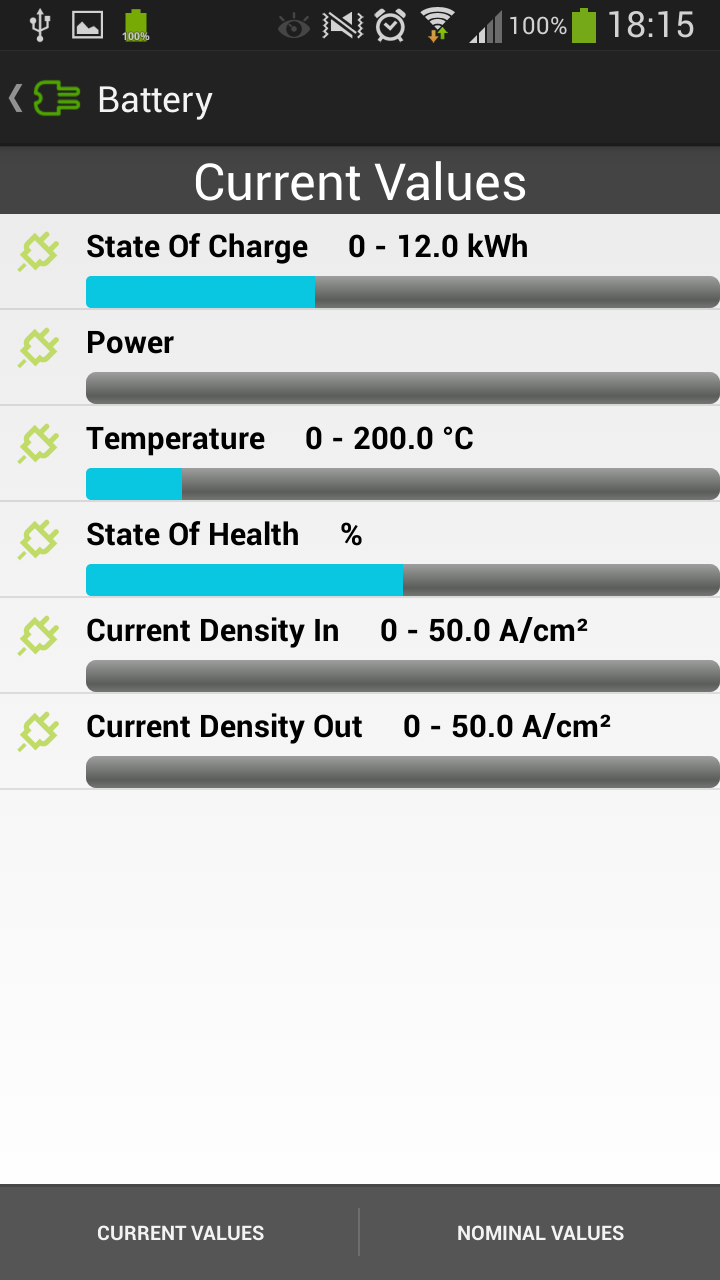
\includegraphics[width=\textwidth]{assets/mobile-app-battery-var.png}
		\caption{Dati variabili della batteria}
		\label{fig:battery-var}
	\end{subfigure}
	\begin{subfigure}{0.45\textwidth}
		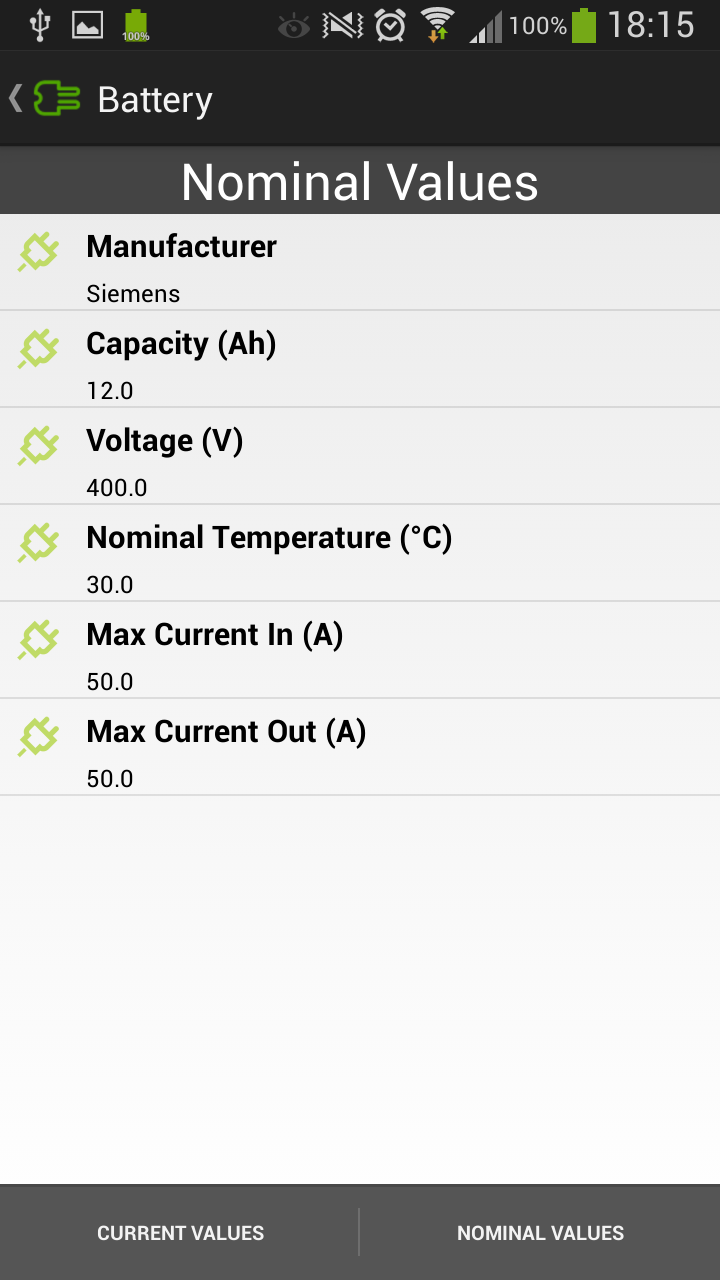
\includegraphics[width=\textwidth]{assets/mobile-app-battery-nom.png}
		\caption{Dati fissi della batteria}
		\label{fig:battery-nom}
    \end{subfigure}
    \begin{subfigure}{0.45\textwidth}
		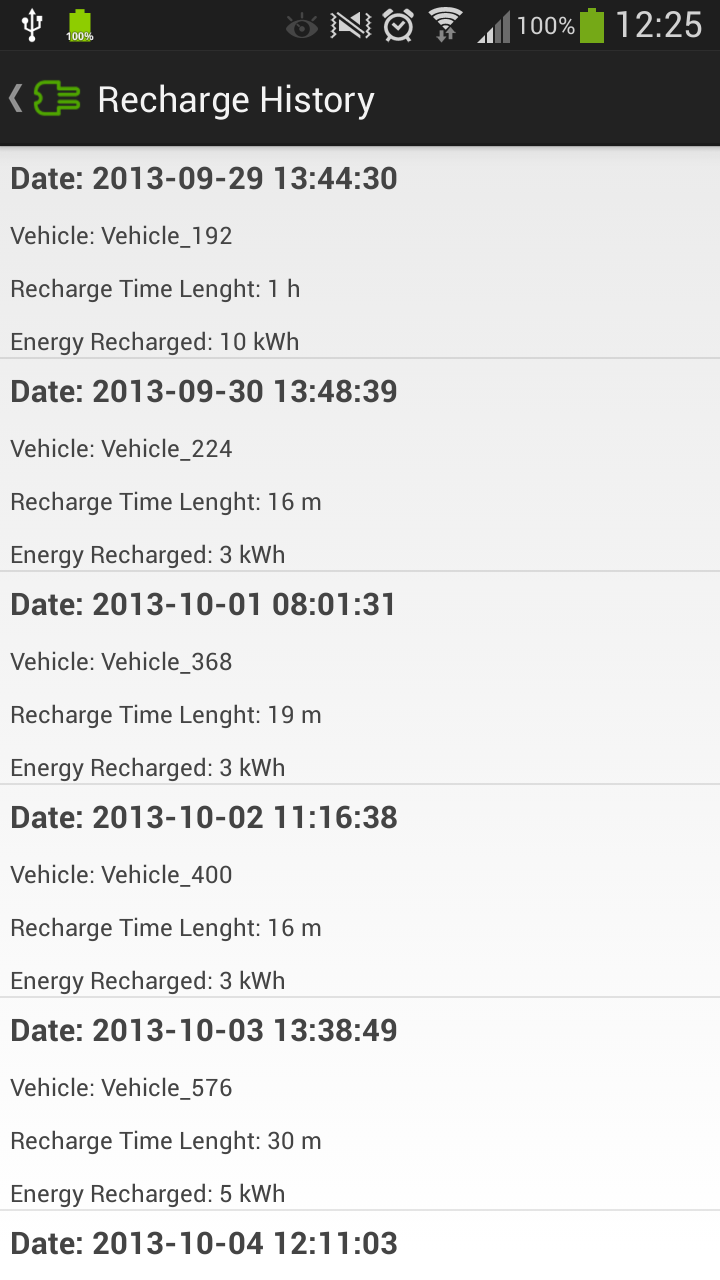
\includegraphics[width=\textwidth]{assets/mobile-app-recharge-history.png}
		\caption{Storia Ricariche}
		\label{fig:recharge-history}
	\end{subfigure}
	\begin{subfigure}{0.45\textwidth}
		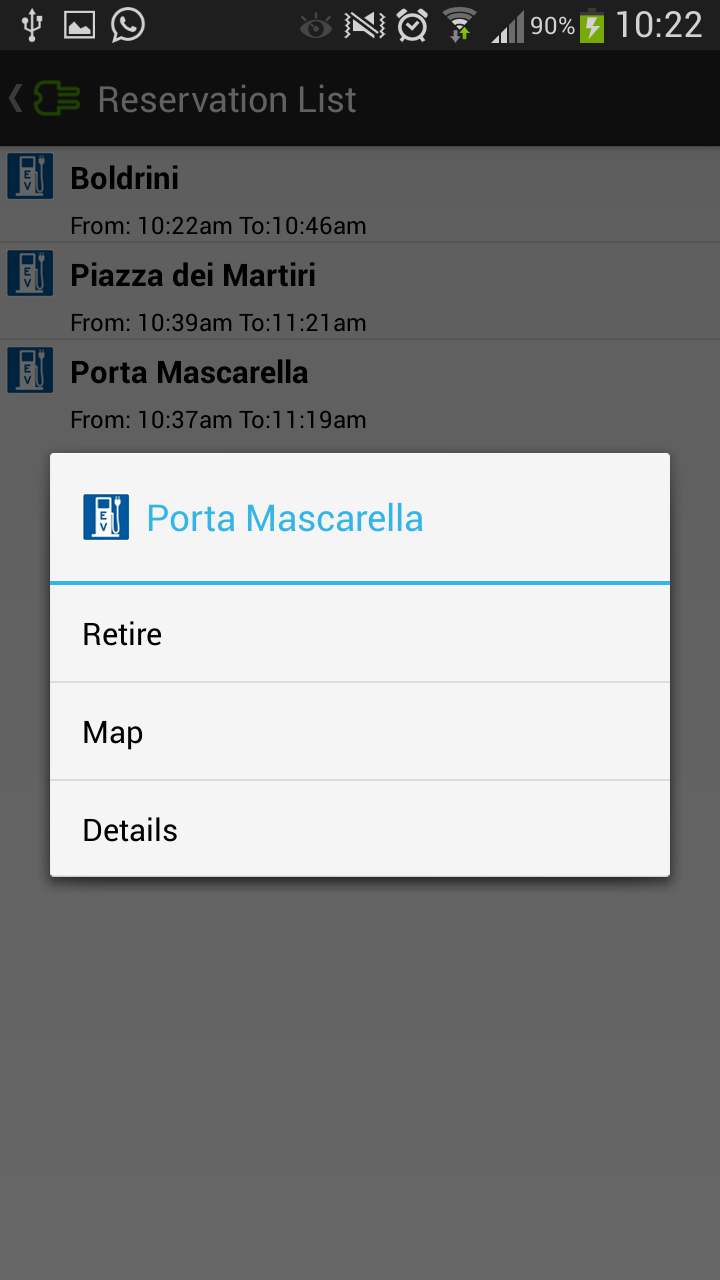
\includegraphics[width=\textwidth]{assets/mobile-app-reservation.png}
		\caption{Selezione Veicolo}
		\label{fig:reservation}
    \end{subfigure}
\end{figure}

\subsection{Effettuare una richiesta di prenotazione}

Per accedere a questa funzionalità bisogna scegliere dal menu principale l'opzione \emph{Reserve}. Ci troveremo davanti alla schermata che ci permette di impostare i parametri necessari a creare una richiesta di prenotazione (~\ref{fig:reservation}). Come si può vedere in figura ~\ref{fig:reservation} io servizio mette a disposizioni svariate opzioni per personalizzare il processo di prenotazione. Essenzialmente in questa schermata viene data una veste grafica al protocollo di richiesta descritto nella sezione ~\ref{sec:protocol}.

\subsubsection{Creazione della richiesta}

La scelta dell'area dentro la quale cercare le colonnine assume di default la posizione del veicolo come punto centrale, nel caso essa non sia disponibile (modalità \emph{Senza Blue\&{}Me}, Sez. ~\ref{subsec:noblueme}) allora l'utente è costretto a sceglierne dalla mappa. Per accedere alla funzione di scelta del punto si clicca sul pulsante \emph{Map} il quale mostra apre la mappa centrata sulla città in cui ci troviamo e tramite un tocco sullo schermo permette di scegliere il punto di interesse (Fig ~\ref{fig:map-chooser}).

Una volta scelto centrata la nostra area di interesse si procede scegliendo il raggio di ricerca. Di default è impostato a 6 e al massimo si può impostare a 15, di più non avrebbe senso visto che in linea di massima si sposta il punto di interesse.

La barra che permette di scegliere la quantità di energia ha come dimensione massima la capacità della batteria. Nell'immagine in Fig. ~\ref{fig:reservation} abbiamo una batteria con capacità 40kWh e una quantità di energia residua di 12kWh, questo si capisce dal colore rosso del numero a destra della barra che indica che stiamo tentando di acquistare 0kWh. Spostando la barra verso destra andremo a indicare fino a che punto volgiamo ricaricare la batteria, il numero a destra a questo punto diventa nero. Non si può procedere finché non si acquista almeno 1kWh. 
Nel caso in cui la capacità e la quantità di carica non siano disponibili allora viene data la possibilità di scegliere qualunque quantità di energia, l'utente viene però messo in guardia del fatto che potrebbe acquistare più energia di quella che può contenere la batteria del veicolo.

L'ultimo parametro da impostare è l'intervallo di tempo in cui siamo disposti a ricaricarci. Di default viene proposto un lasso temporale di 3 ore. È possibile variarlo premendo sui pulsanti nel quale è scritta la data i quali mostreranno un calendario e un selettore di orario. Ovviamente sono stati messi dei controlli che impediscono di mettere orari incoerenti come ora di inizio successiva a quella di fine.

A questo punto possiamo inviare la richiesta premendo l'apposito pulsante in alto a destra.

\subsubsection{Scelta della risposta}

In seguito all'invio della richiesta viene mostrato all'utente un messaggio che invita ad attendere la risposta. Nel caso la richiesta sia fallita allora l'utente viene allertato e rimandato nella schermata di prenotazione con l'invito di cambiare i parametri.

In caso di successo viene mostrata una schermata con tutte le opzioni di ricarica restituite dal servizio cittadino. Come si può vedere in Fig. ~\ref{fig:charge-options} vengono fornite diverse informazioni per ognuna di esse:

\begin{itemize}
	\item Nome del GCP presso cui avverrà la ricarica.
	\item Distanza reale dal GCP, calcolata grazie alla libreria UniboGeoTools.
	\item Orario e prezzo della ricarica.
	\item Energia stimata per raggiungere la colonnina.
	\item Dislivello in salita e in discesa.
\end{itemize}

Le informazioni sul profilo altimetrico ed il contributo energetico vengono mostrate in una schermata a parte accessibile tramite un apposito menu visualizzabile tenendo premuta a lungo un opzione di ricarica (Fig. ~\ref{fig:charge-options-menu}), questo aspetto verrà approfondito in una sezione a parte (~\ref{subsec:altimetry}).

Viene data inoltre la possibilità di eseguire operazioni di ordinamento delle varie ricariche in base ai parametri sopra elencati ovvero: distanza, prezzo, orario, contributo energetico ecc.. Infine volendo si possono guardare le opzioni di ricarica sulla mappa. Premendo su una di esse viene disegnato il percorso necessario ad arrivarci con la particolarità che i tratti in salita sono colorati di rosso, quelli in discesa di verde e infine quelli in pianura di grigio. Le caratteristiche della mappa sono comunque approfondite nella Sez. ~\ref{subsec:map}.

Scegliendo l'opzione di ricarica viene eseguita la parte restante del protocollo, e nel caso in cui sia ancora valida allora verremo mandati alla schermata che presenta le prenotazioni attive per l'utente.

\begin{figure}
	\centering
	\begin{subfigure}{0.45\textwidth}
		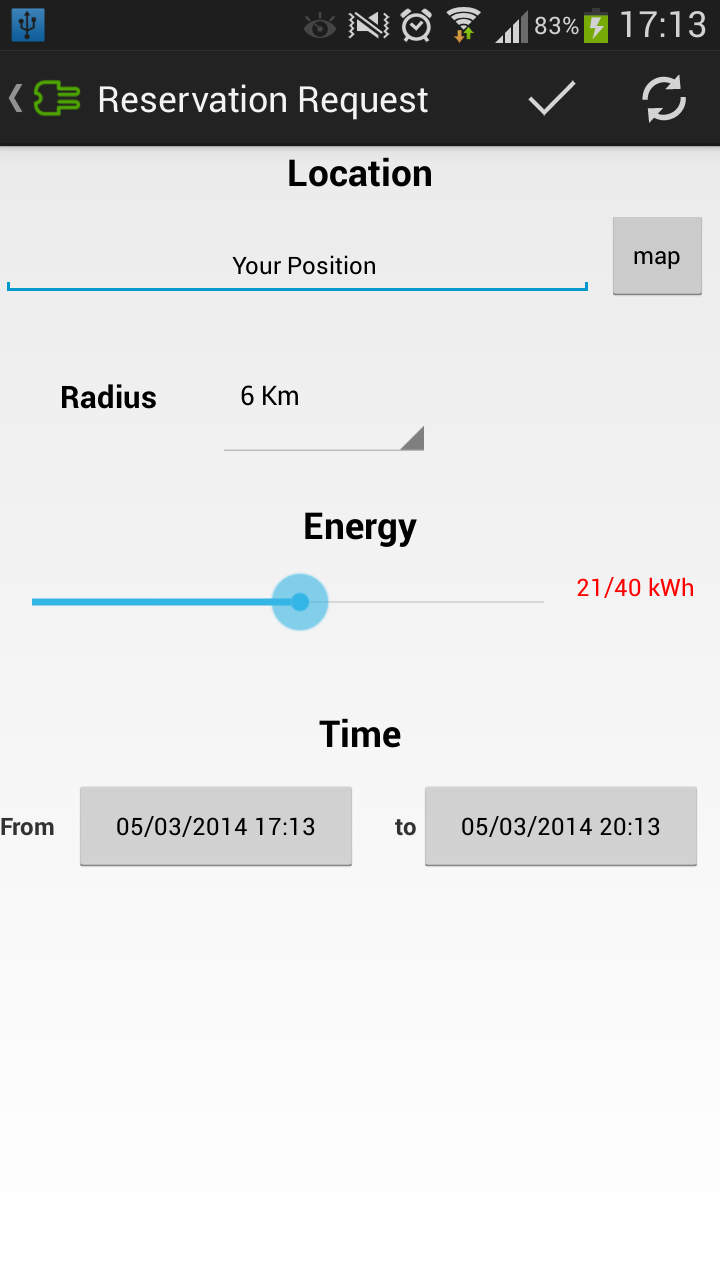
\includegraphics[width=\textwidth]{assets/mobile-app-charge-request.png}
		\caption{Inserimento Prenotazione}
		\label{fig:reservation}
	\end{subfigure}
	\begin{subfigure}{0.45\textwidth}
		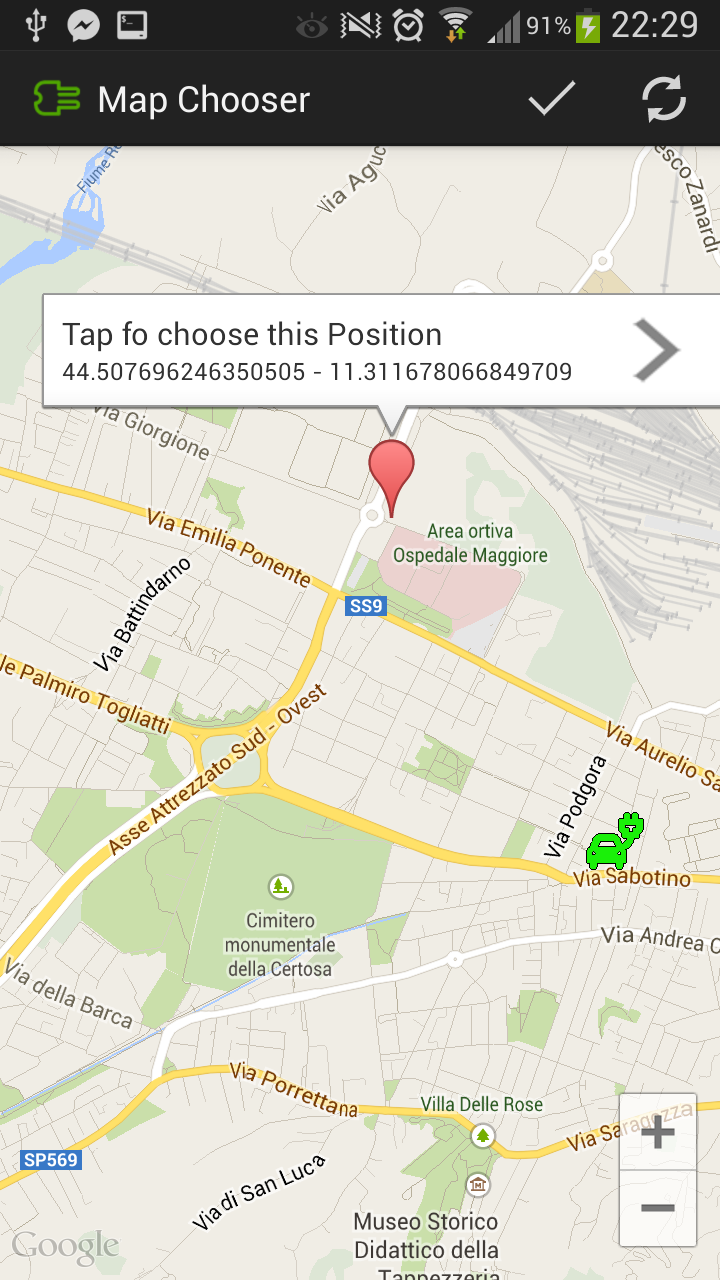
\includegraphics[width=\textwidth]{assets/mobile-app-map-chooser.png}
		\caption{Scelta di un punto nella mappa}
		\label{fig:map-chooser}
	\end{subfigure}
	\begin{subfigure}{0.45\textwidth}
		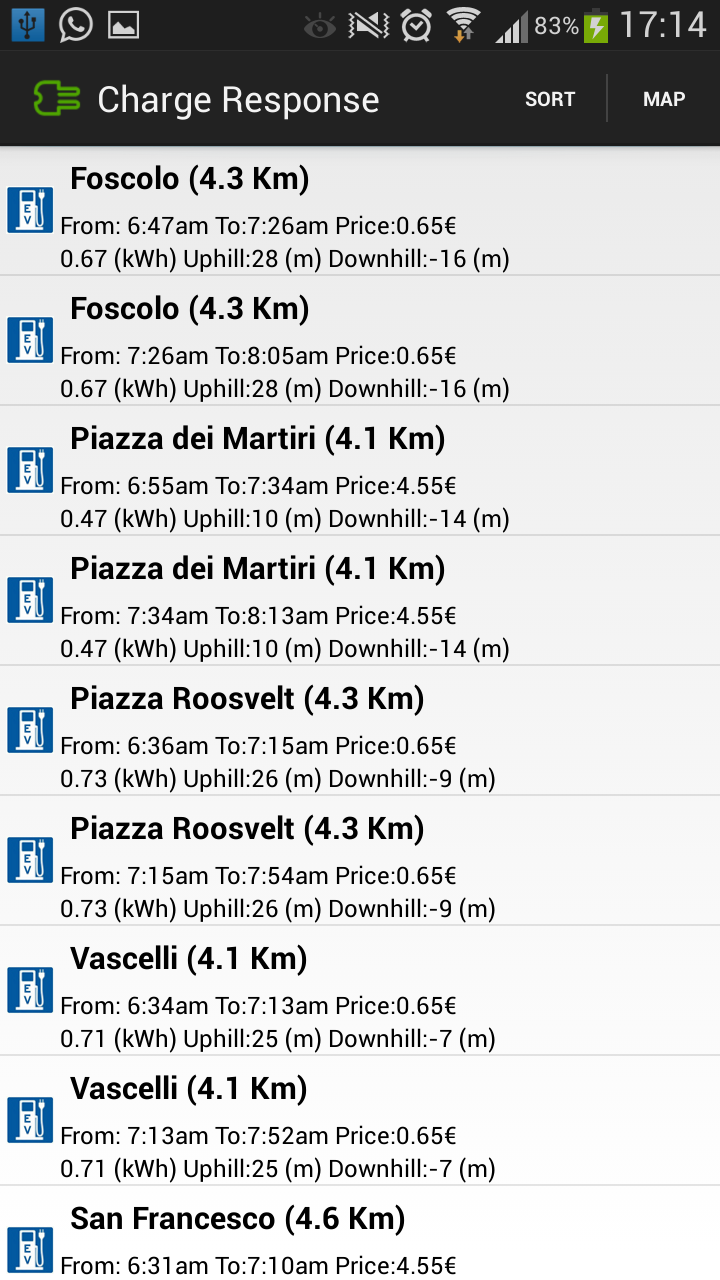
\includegraphics[width=\textwidth]{assets/mobile-app-charge-options.png}
		\caption{Visualizzazione opzioni di ricarica}
		\label{fig:charge-options}
    \end{subfigure}
	\begin{subfigure}{0.45\textwidth}
		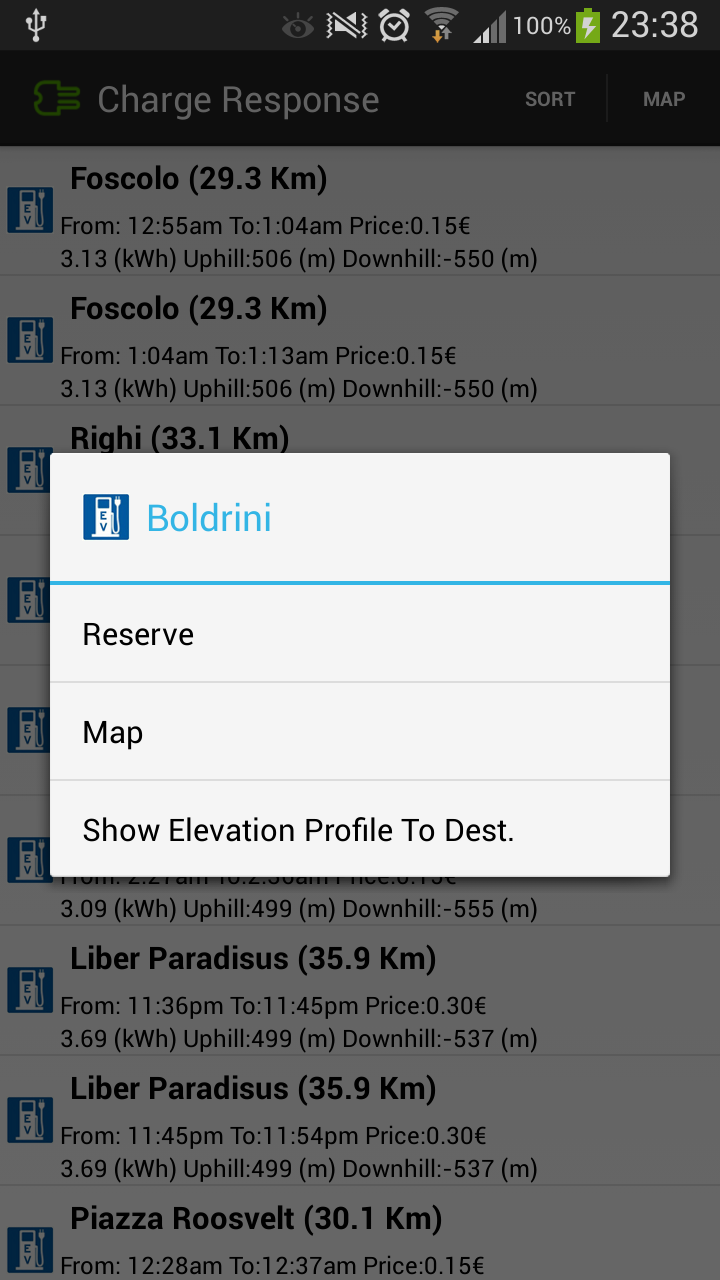
\includegraphics[width=\textwidth]{assets/mobile-app-charge-options-menu.png}
		\caption{Menu opzioni di ricarica}
		\label{fig:charge-options-menu}
    \end{subfigure}
\end{figure}

\subsection{Profilo Altimetrico e Contributo Energetico}\label{subsec:altimetry}

Il profilo altimetrico è una delle feature più innovative introdotte nell'applicazione. Può rivelarsi di fondamentale importanza nelle scelte dell'utente il quale, grazie ad essa, potrà scegliere il percorso migliore al fine di raggiungere la sua destinazione. Come vedremo nella sezione relativa al modello della batteria (\ref{sec:battery}), i veicoli elettrici hanno la possibilità di recuperare energia grazie alla frenata rigenerativa e al recupero in discesa. Questo significa che scegliere una strada con molti tratti in discesa può portare un recupero di energia non indifferente. 

La libreria UniboGeoTools, usata a questo scopo, permette inoltre di fare delle stime sull'energia necessaria a percorre un determinato tratto di strada. Queste informazioni sono mostrate nella schermata \emph{Elevation Profile}:

\begin{itemize}
	\item \textbf{Path Altimetry Summary}: Informazioni riassuntive sul viaggio che stiamo per intraprendere. Come si può vedere in Fig. ~\ref{fig:altimetry-1}, al di la delle informazioni di destinazione, distanza e peso, viene fornita una stima sull'energia totale che impiegherà il veicolo a raggiungere la destinazione, insieme alle informazioni su quanta discesa, salita e pianura compongo il percorso.
	\item \textbf{Cumulative Altimetry Offset}: In questo riquadro vengono fornite informazioni sul dislivello che caratterizza il percorso (Fig ~\ref{fig:altimetry-1}).
	\item \textbf{Average Slope}: Fornisce informazioni sulla pendenza media che caratterizza il percorso. Importante in quanto, come detto prima, una pendenza molto elevata può portare ad elevati consumi oppure a un ricavo di energia (Fig ~\ref{fig:altimetry-1}).
	\item \textbf{Max Slope}: Fornisce informazioni di massima sulla pendenza del percorso, ovvero la pendenza massimo che troveremo in salita e in discesa (Fig ~\ref{fig:altimetry-2}).
	\item \textbf{Elevation Dependent Energy Ref}: Informazioni sul contributo energetico impiegato per vincere il dislivello. A tal scopo viene utilizzata l'energia potenziale gravitazionale (Fig ~\ref{fig:altimetry-2}).
	\item \textbf{Energy Profile for Path Lenght}: Energia impiegata per percorrere il tragitto. Mentre nel caso precedente veniva preso in considerazione unicamente il dislivello qui viene considerata anche la distanza che ci separa dalla destinazione (Fig ~\ref{fig:altimetry-2}).
	\item \textbf{Altitude Graph}: Grafico che mostra il profilo altimetrico che ci separa dalla destinazione. I tratti in discesa sono in verde mentre quelli in salita in rosso (Fig ~\ref{fig:altimetry-3}).
\end{itemize} 
\noindent
Ulteriori informazioni sul profilo altimetrico vengono date sulla mappa aspetto approfondito nella Sez. ~\ref{subsec:map}.


\subsection{Mappa}\label{subsec:map}


\begin{figure}
	\centering
	\begin{subfigure}{0.45\textwidth}
		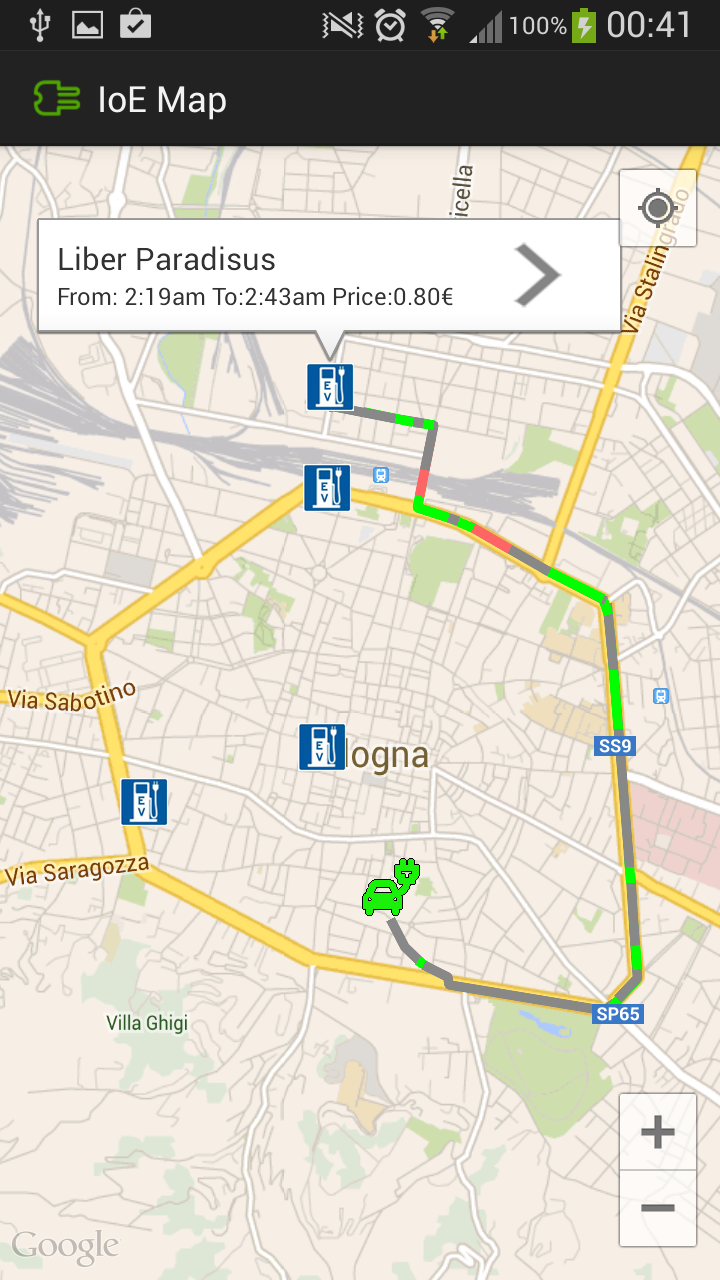
\includegraphics[width=\textwidth]{assets/mobile-app-map.png}
		\caption{Mappa con Profilo Altimetrico}
		\label{fig:map-altimetry}
	\end{subfigure}
	\begin{subfigure}{0.45\textwidth}
		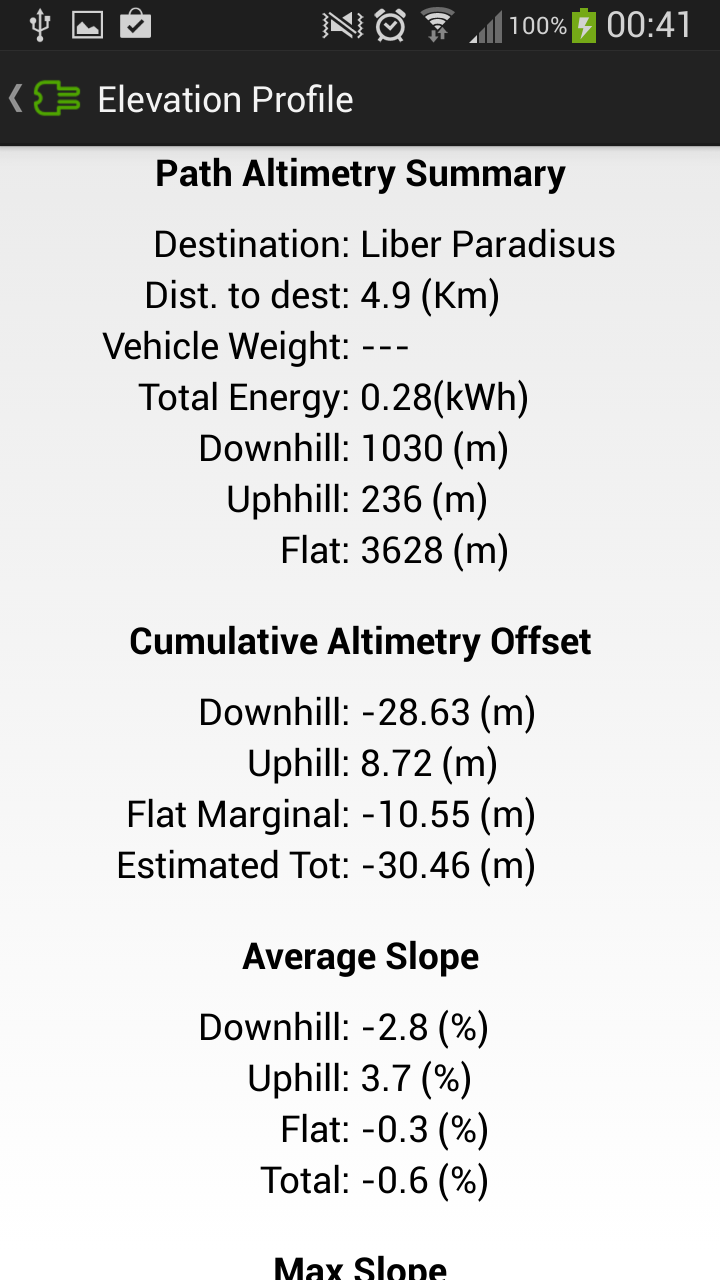
\includegraphics[width=\textwidth]{assets/mobile-app-altimetry-1.png}
		\caption{Scelta di un punto nella mappa}
		\label{fig:altimetry-1}
	\end{subfigure}
	\begin{subfigure}{0.45\textwidth}
		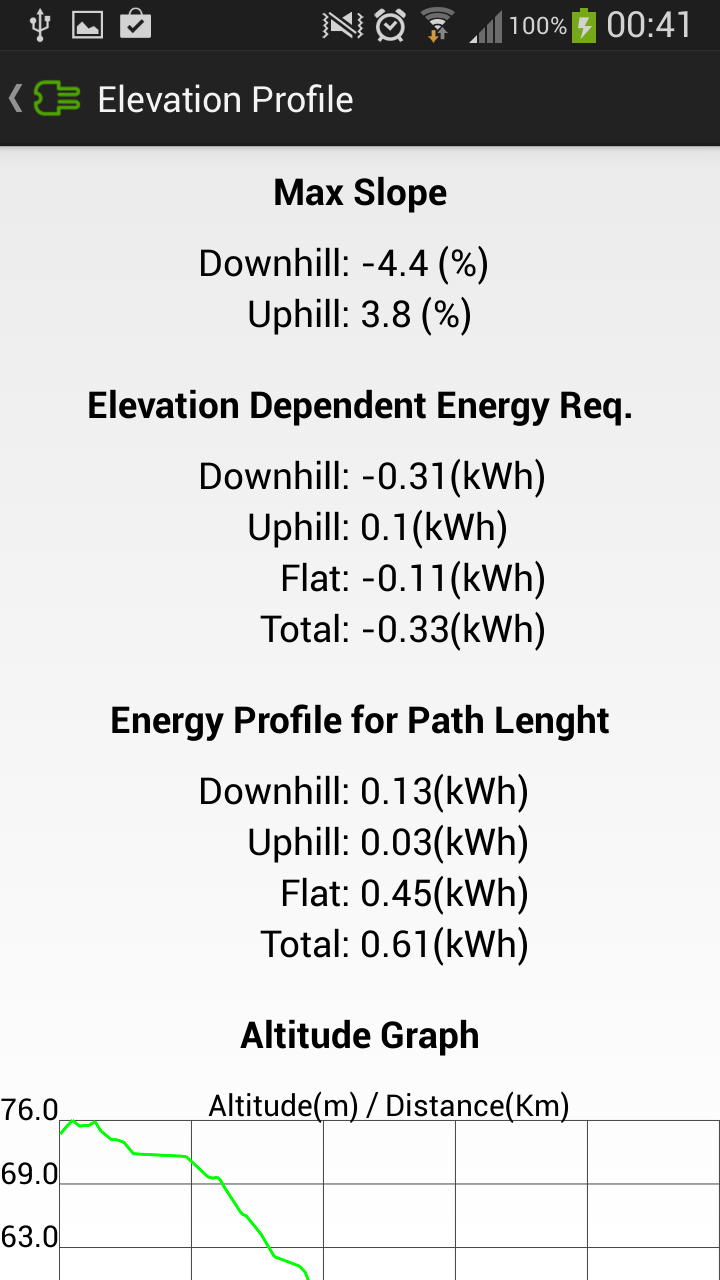
\includegraphics[width=\textwidth]{assets/mobile-app-altimetry-2.png}
		\caption{Visualizzazione opzioni di ricarica}
		\label{fig:altimetry-2}
    \end{subfigure}
	\begin{subfigure}{0.45\textwidth}
		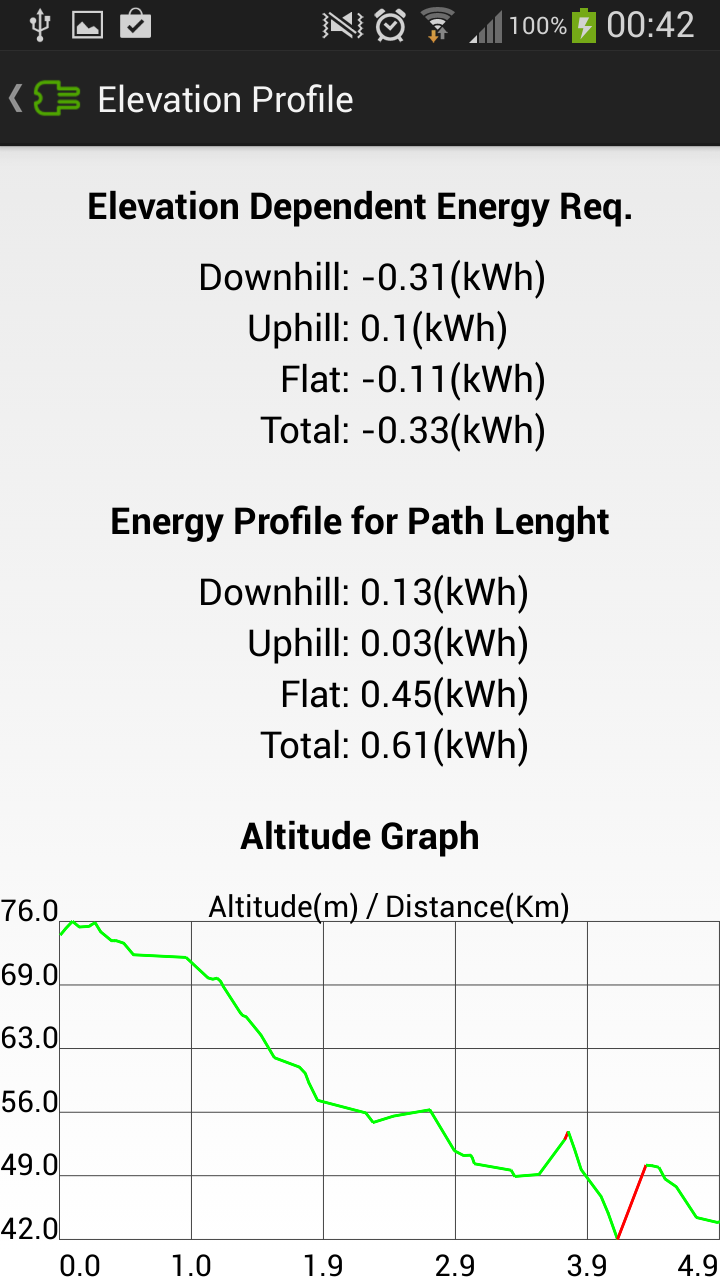
\includegraphics[width=\textwidth]{assets/mobile-app-altimetry-3.png}
		\caption{Menu opzioni di ricarica}
		\label{fig:altimetry-3}
    \end{subfigure}
\end{figure}

\section{Activities}
